\section{R-trees}
\label{sec:rtree}

\subsection{R-trees in general}
From \textcite{rtree}, an R-tree is a tree structure composed of nodes containing multi-dimensional data, facilitating range searches accross multiple dimensions. There are many variations of these trees: R-tree, $\text{R}^+$-tree, $\text{R}^*$-tree, and Hilbert R-tree. There are also two main categories of R-trees, dynamic and static. Dynamic trees are best suited for dynamic data (many writes) and static trees for static data (few writes). This section will discuss R-trees generally, and delve further into some variants that are especially relevant for this thesis.

Key to all R-trees is the Minimum Bounding Rectangle (MBR), as each node in the tree is defined by this. It represent the range of all dimensions for that node and its child nodes. For leaf nodes the MBR represents the range of its data. A leaf node typically references data points rather than storing them directly in the tree. R-trees generally try to minimize the area of MBRs to improve query processing \cite{rtree}. Figure \ref{fig:rtree} illustrates the node hierarchy within an R-tree, with the associated MBRs depicted in figure \ref{fig:mbrs}. An R-tree can be used to efficiently retrieve references to all data points within a certain range from a large dataset. This is known as a range (or window) query \cite{rtree}. When querying a range, only nodes with MBRs overlapping with the range are considered, potentially reducing the number of invoked nodes, and thereby also the number of accessed data points.

The $\text{R}^*$-tree takes three new criterion into consideration to improve performance during query processing from that of an R-tree: MBR overlap minimization, MBR margin minimization, and storage utilization \cite{rtree}. Reducing overlap leads to fewer paths being pursued during query processing. Margin minimization makes MBRs more quadratic which makes them fit better together, indirectly improving area minimization. Low storage utilization leads to more nodes being invoked during a query. Therefore it tries to have high storage utilization by keeping the height of the tree low. Additionally larger space utilization leads to less storage space being used. The $\text{R}^*$-tree is considered the most robust variant, suitable to many applications \cite{rtree}.

\begin{figure}
    \centering
    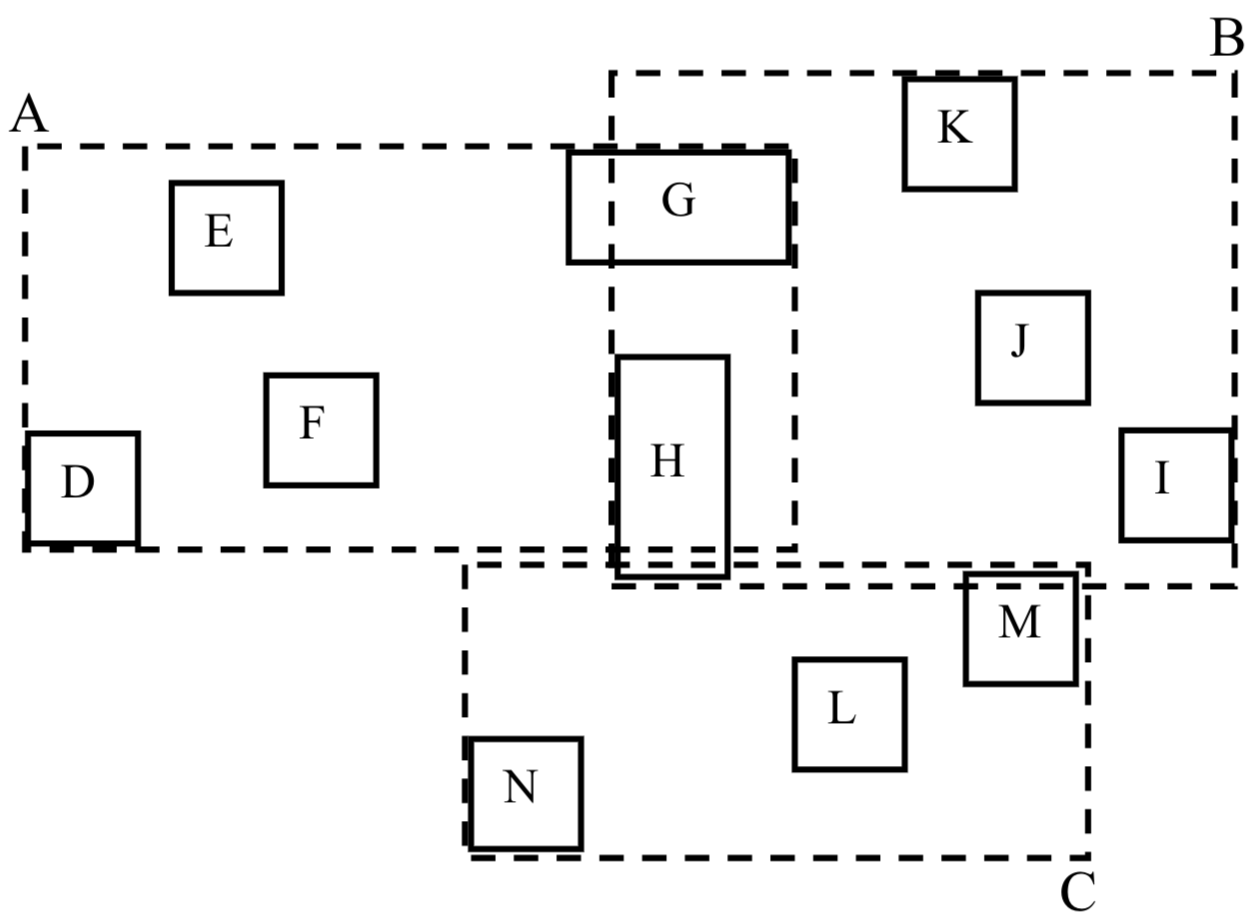
\includegraphics[width=0.5\linewidth]{./figures/mbrs.png}
    \caption{An example of data MBRs and their MBRs, from \cite{rtree}.}
    \label{fig:mbrs}
\end{figure}
\begin{figure}
    \centering
    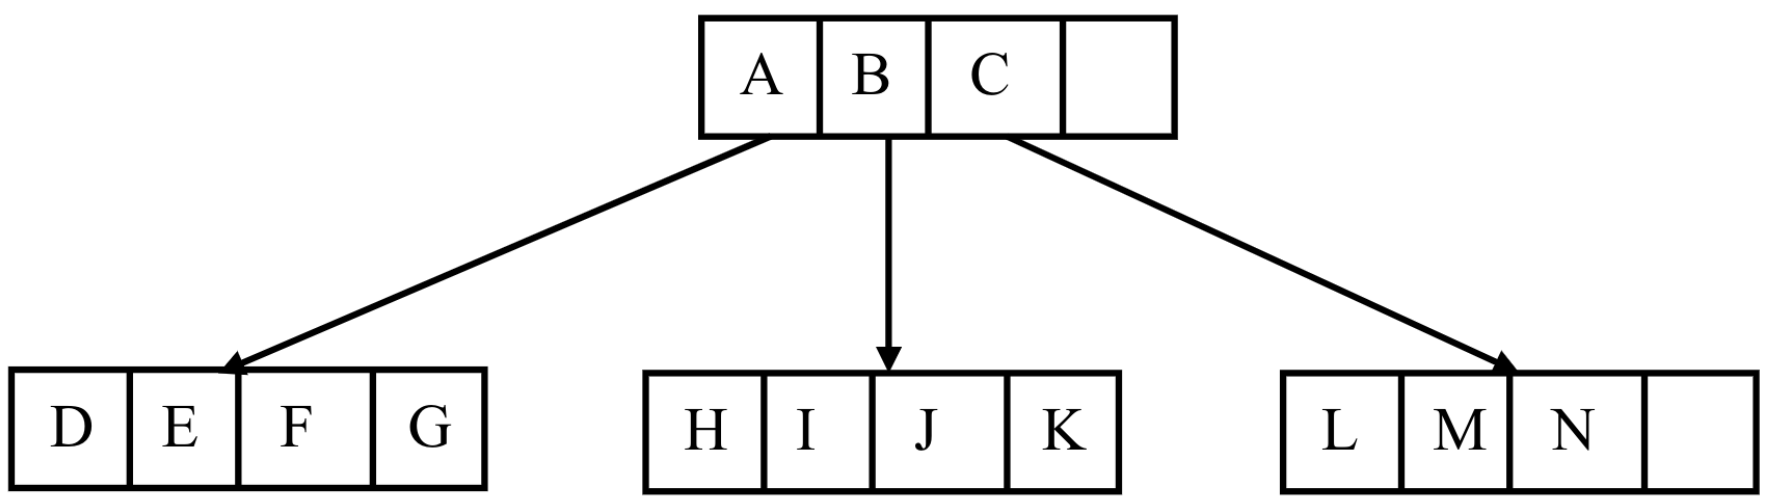
\includegraphics[width=\linewidth]{./figures/rtree.png}
    \caption{The corresponding R-tree, from \cite{rtree}.}
    \label{fig:rtree}
\end{figure}

\subsection{Hilbert R-tree}
The Hilbert R-tree exists in both dynamic and static variants, Hilbert R-tree, and Packed Hilbert R-tree, respectively. The packed variant performed significantly better than $\text{R}^*$-tree for point and range queries, from empirical studies \cite{rtree}. One drawback of the Packed Hilbert R-tree is that it struggles with many dimentions. However spatial data typically only uses one to three dimensions: x, y, and z. Therefore it is well suited for static spatial data.

To explain the Packed Hilbert R-tree the (dynamic) Hilbert R-tree must first be discussed. A Hilbert R-tree separates itself from other variants with the MBR selection. It utilizes Hilbert curves to generate MBRs for nodes. A Hilbert curve is a space-filling curve that can traverse every point in higher-dimensional space. This property allows for the mapping of two-dimensional values to one-dimensional values by drawing the curve in two dimensions and assigning ascending values to the points along the curve, see figure \ref{fig:hilbert} for Hilbert curves with corresponding values. These values are referred to as Hilbert values. Hilbert curves have the characteristic such that elements close in space will also be close in Hilbert values \cite{rtree}. By sorting MBRs based on the Hilbert value of the rectangle centroids, MBRs with minimal overlap can be created.

The Packed version uses a packing algorithm that provides a better MBR selection. This requires bulk loading all data, this allows for a better sorting and creation of MBRs. However, this process is resource intensive and too many bulk loads can lead to worse performance. The Packed Hilbert R-tree achieves a storage utilization of nearly 100\%, whereas the static counterpart had a storage utilization of nearly 70\% \cite{rtree}.

\begin{figure}[t]
    \centering
    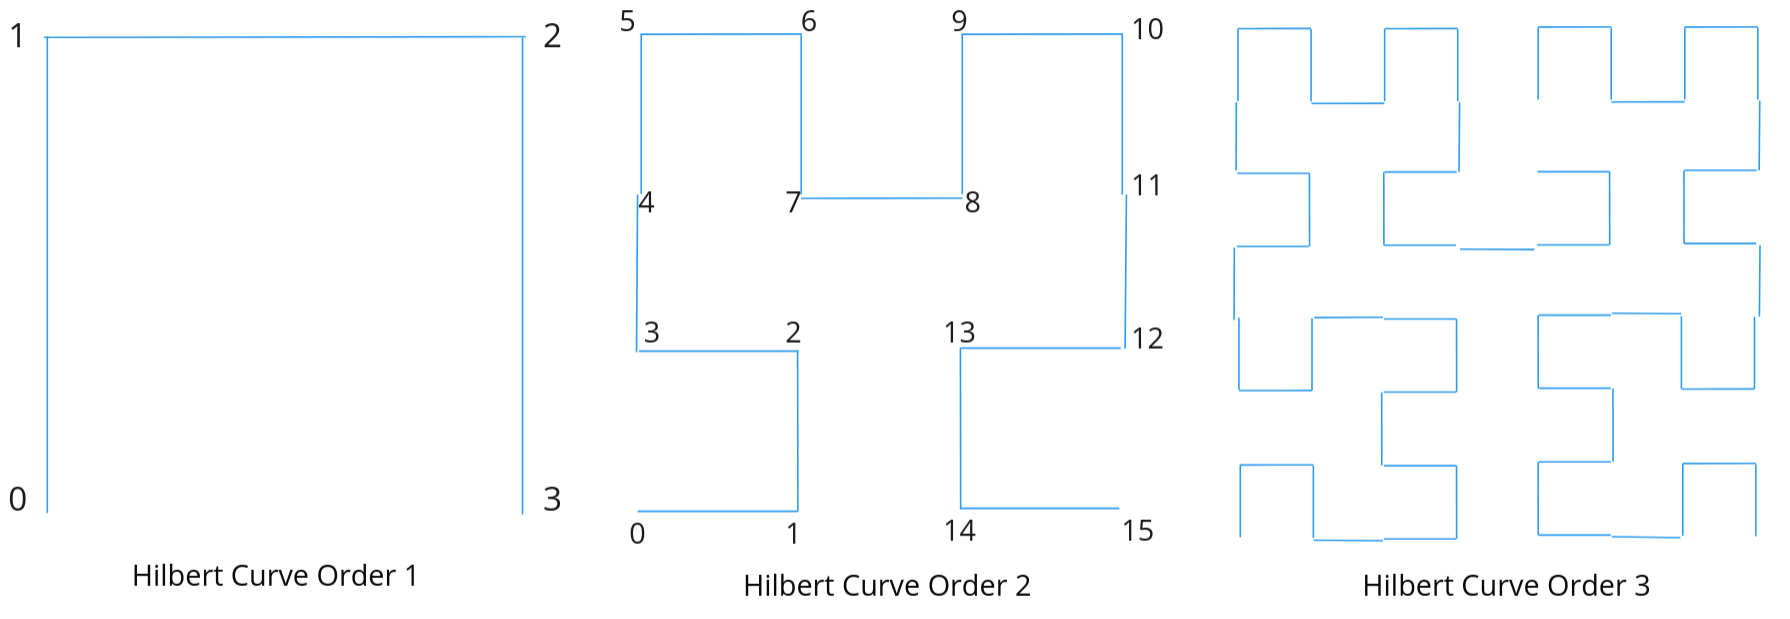
\includegraphics[width=\linewidth]{./figures/hilbert_orders.png}
    \caption{Showing Hilbert Curves of orders 1, 2, and 3.}
    \label{fig:hilbert}
\end{figure}

% \section{Range search}
% - how to 